\documentclass[onecolumn, draftclsnofoot,10pt, compsoc]{IEEEtran}
\usepackage{graphicx}
\usepackage{url}
\usepackage{setspace}
\usepackage{pstricks-add}
\usepackage{float}

\usepackage{geometry}
\geometry{textheight=9.5in, textwidth=7in}

% 1. Fill in these details
\def \CapstoneTeamName{		AKA Robotics}
\def \CapstoneTeamNumber{		13}
\def \GroupMemberOne{     Arthur Shing}
\def \GroupMemberTwo{			Kevin Talik}
\def \GroupMemberThree{   Anish Asrani}
\def \CapstoneProjectName{		How to Make an Effective Robot Comedian}
\def \CapstoneSponsorCompany{	Oregon State University}
\def \CapstoneSponsorPerson{		Heather Knight}

% 2. Uncomment the appropriate line below so that the document type works
\def \DocType{		%Problem Statement
				%Requirements Document
				%Technology Review
				Design Document
				%Progress Report
				}
			
\newcommand{\NameSigPair}[1]{\par
\makebox[2.75in][r]{#1} \hfil 	\makebox[3.25in]{\makebox[2.25in]{\hrulefill} \hfill		\makebox[.75in]{\hrulefill}}
\par\vspace{-12pt} \textit{\tiny\noindent
\makebox[2.75in]{} \hfil		\makebox[3.25in]{\makebox[2.25in][r]{Signature} \hfill	\makebox[.75in][r]{Date}}}}
% 3. If the document is not to be signed, uncomment the RENEWcommand below
\renewcommand{\NameSigPair}[1]{#1}

%%%%%%%%%%%%%%%%%%%%%%%%%%%%%%%%%%%%%%%
\begin{document}

\bstctlcite{IEEEexample:BSTcontrol}
\begin{titlepage}
    \pagenumbering{gobble}
    \begin{singlespace}
        \hfill 
        % 4. If you have a logo, use this includegraphics command to put it on the coversheet.
        %\includegraphics[height=4cm]{CompanyLogo}   
        \par\vspace{.2in}
        \centering
        \scshape{
            \huge CS Capstone \DocType \par
            {\large\today}\par
            \vspace{.5in}
            \textbf{\Huge\CapstoneProjectName}\par
            \vfill
            {\large Prepared for}\par
            \Huge \CapstoneSponsorCompany\par
            \vspace{5pt}
            {\Large\NameSigPair{\CapstoneSponsorPerson}\par}
            {\large Prepared by }\par
            Group\CapstoneTeamNumber\par
            % 5. comment out the line below this one if you do not wish to name your team
            \CapstoneTeamName\par 
            \vspace{5pt}
            {\Large
                \NameSigPair{\GroupMemberOne}\par
                \NameSigPair{\GroupMemberTwo}\par
                \NameSigPair{\GroupMemberThree}\par
            }
            \vspace{20pt}
        }
        \begin{abstract}
        \end{abstract}     
    \end{singlespace}
\end{titlepage}
\newpage
\pagenumbering{arabic}
\tableofcontents
% 7. uncomment this (if applicable). Consider adding a page break.
%\listoffigures
%\listoftables
\clearpage

% 8. now you write!
\section{Introduction}
  This is an intro

\section{Adaptation}
  We hypothesize that to make the set the most effective, the comedian needs to transition to topics; this is dependent on the audience response to jokes. The goal of this portion of the project is to determine if adapting the content from the audience response will enhance the overall performance of the comedian. In the beginning of the set, the comedian will present an "initialization" procedure, known as the "Seed Jokes" to test the response of the audience to different jokes. Depending on their response, the comedian will transition to a theme that is evaluated to be the best fit. The robot comedian will have many jokes to choose from that contain different material, but not all audiences will like all of the jokes. Figure 1 shows how the theme will be chosen from a set of up to \textit{k} themes. The closing joke will be a subset of all jokes that might be stronger joke than some of the others, and is helpful in ending the show on a stronger note. It may be a stretch to optimize with traditional machine learning because there may not be a large enough data set to adequately return results. Primarily, this algorithm needs to choose an optimal joke to fill the performance, while taking the audience into account.

\begin{figure}[H]
  \centering
  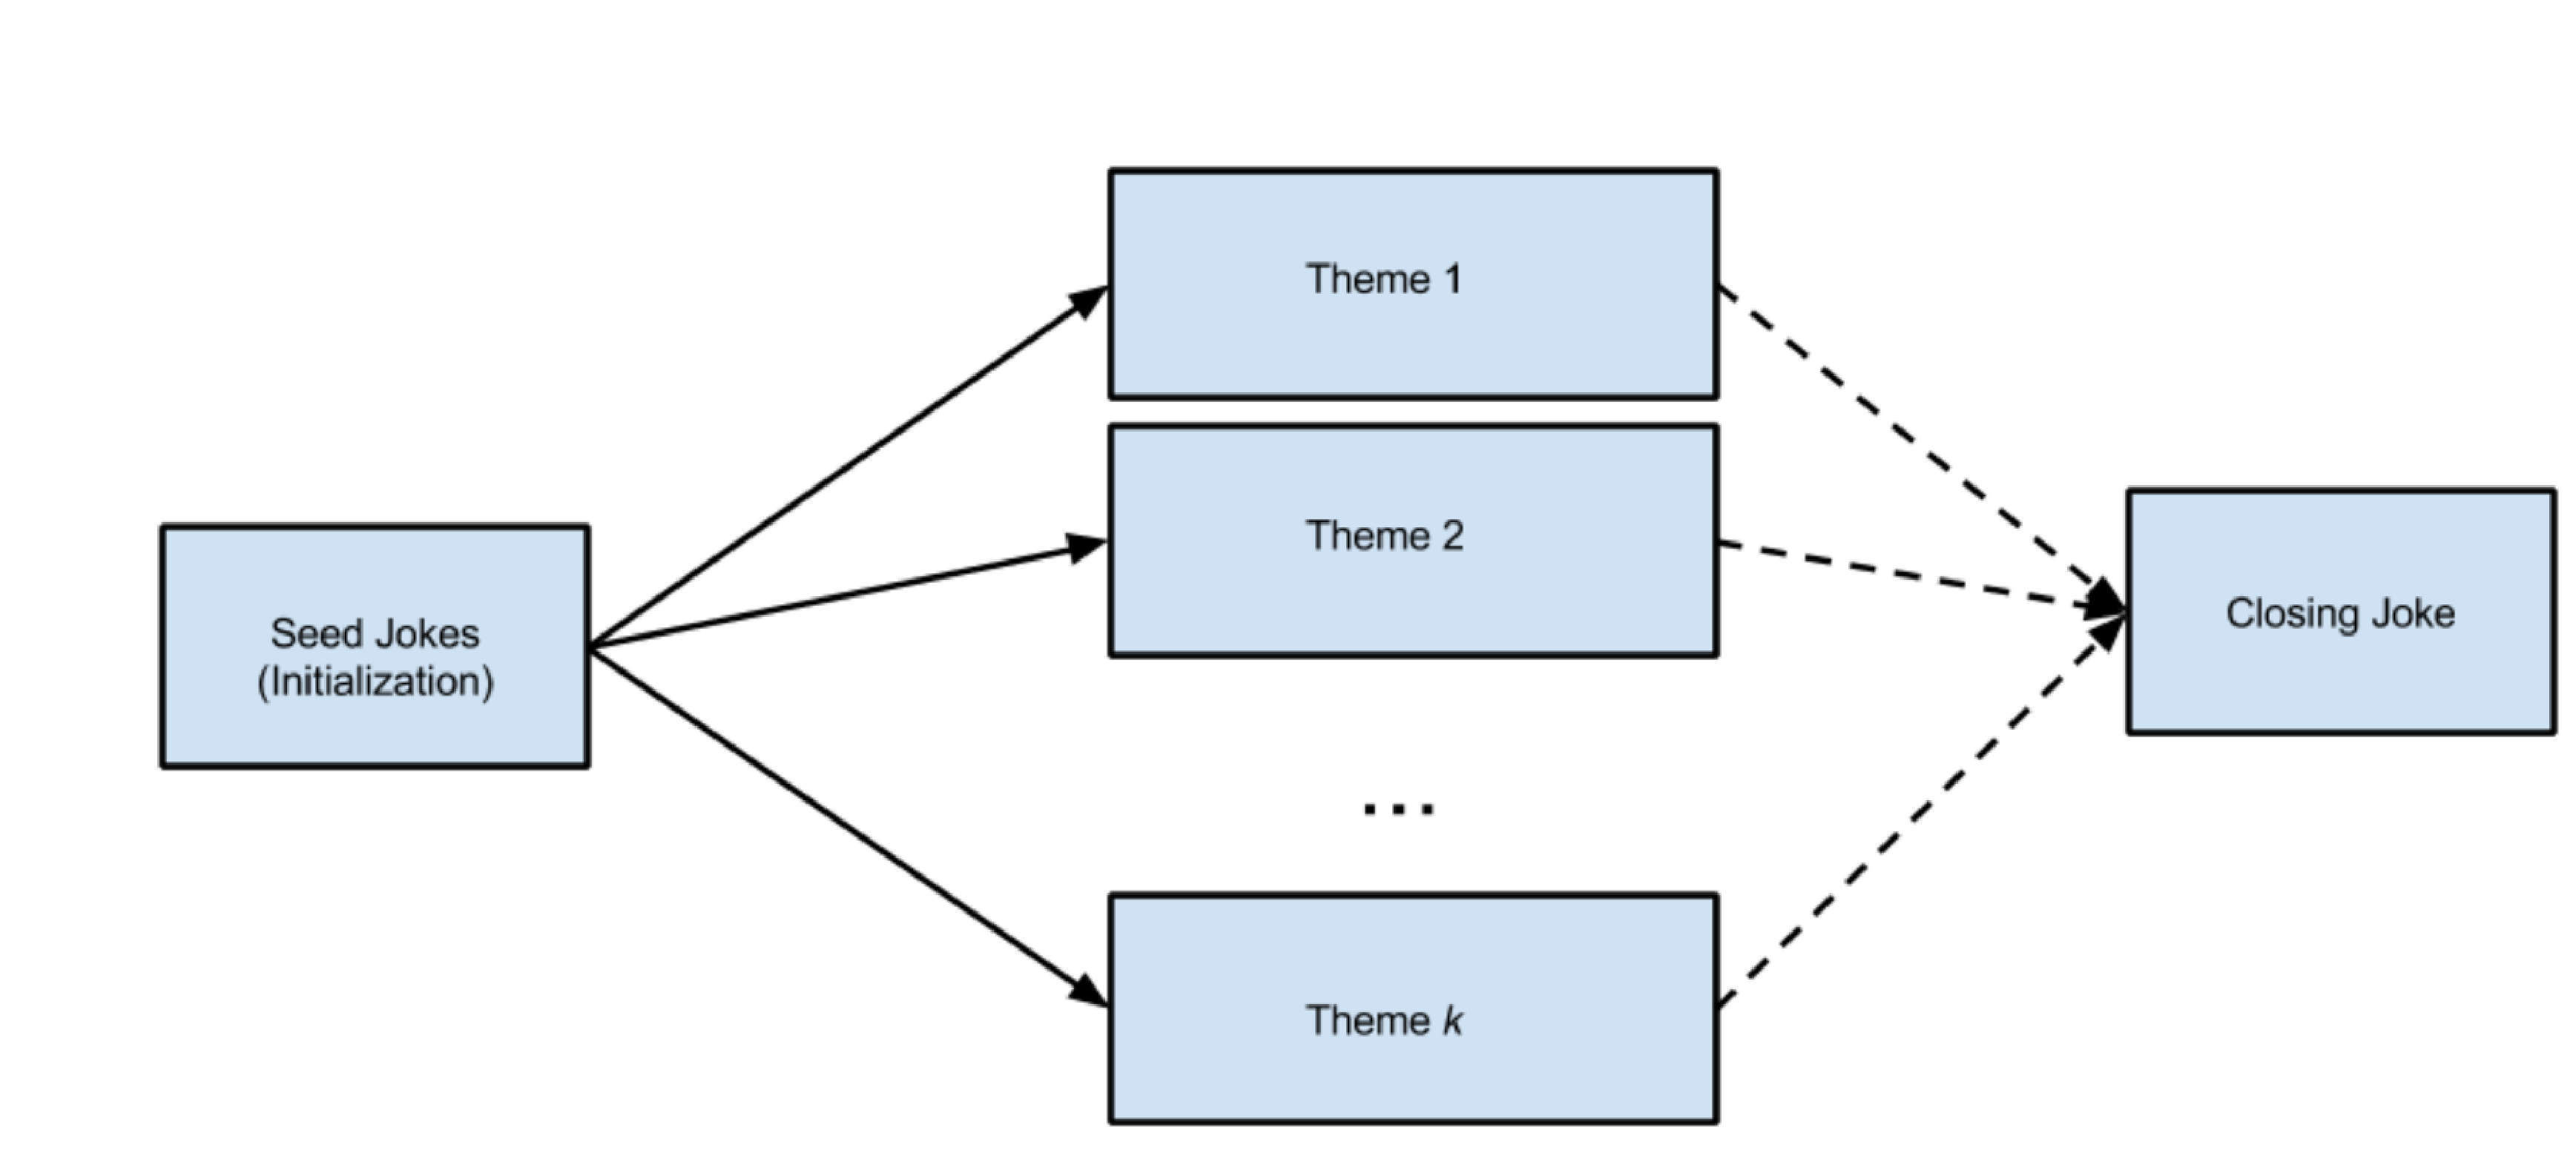
\includegraphics[width=0.75\textwidth,height=0.75\textheight,keepaspectratio]{fig0}
  \caption{This shows how algorithm will have up to \textit{k} Themes to choose from, determined from the seed joke. The closing joke is a subset of all jokes, and may be outside of a specific theme. There could be different spanning trees of performances that end at the same closing joke}
\end{figure}

Figure 2 depicts how a joke will be represented by the robot. It will perform the joke, collect audience feedback information, and branch to the joke that will best fit the response. For example, if two of the seed jokes are about "food" and "mindfulness", the performance will branch to the respective theme that matches the audience response (Branch 1 or Branch 2). If jokes with a theme of "food" are not landing with the audience, the algorithm will need to know when to transition to a new theme, or when to end the set. When the robot tells a joke, it needs to be able to analyze the feedback and choose the next joke to perform. This needs to be done quickly, so that the robot is not spending noticeable time (to the audience) choosing a joke. There may not be a lot of jokes to choose from, but the choice needs to be made fast.

Generally, the performance will have three parts: The Seed Jokes, Middle Content, and Closing Joke. The Seed will influence the Middle Content, which will be chosen themed jokes and basis of the show. The Middle Content will transition to the Closing Joke when it is time to end the show. The most work that needs to be done is learning about closing jokes, and their influence on the performance. This final joke needs to reflect the performance that the robot gave.
\begin{figure}[H]
  \centering
  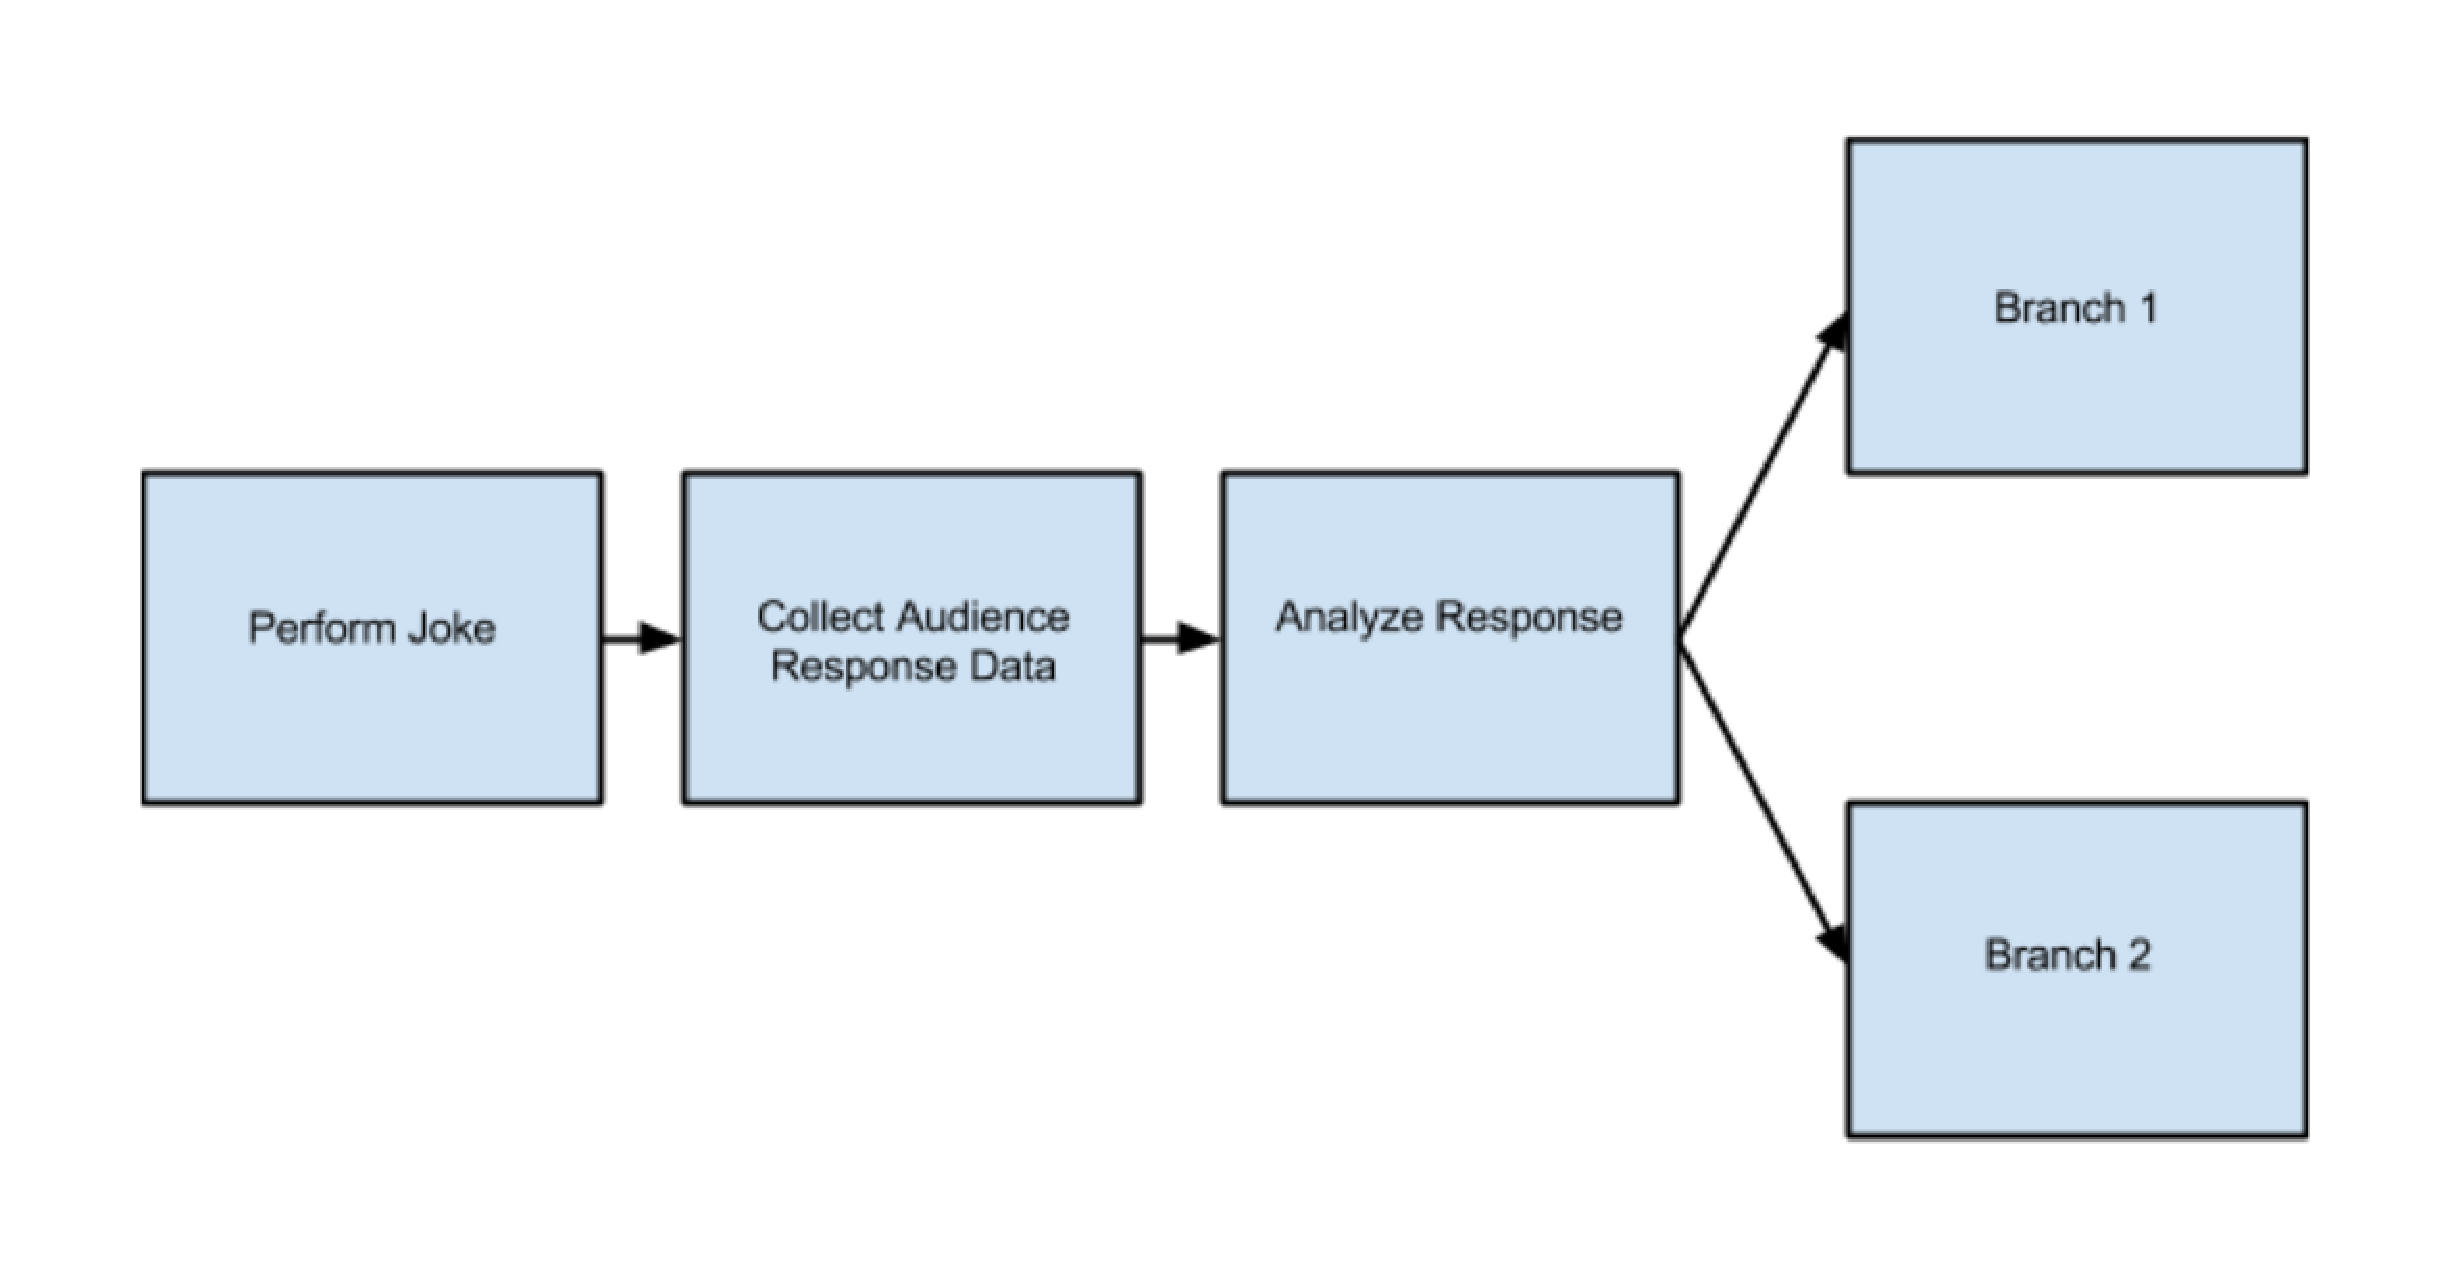
\includegraphics[width=0.75\textwidth,height=0.75\textheight,keepaspectratio]{fig1}
  \caption{}
\end{figure}

\section{Crowd-work}
Crowd-work in a performance includes incorporating the audience and make them feel like they are a part of the show. This can be done in various different ways -  calling out and talking to the audience, listening to the audience and making relevant comments, asking them questions to keep them engaged. We want to analyze the importance of this crowd-work in a robot stand-up comedy performance. 

There are various degrees of this crowd-work we want to test. The first one would be no crowd-work whatsoever. The robot goes about performing its set and may acknowledges its lack of sensing and interaction. The second would be over the top and inaccurate crowd-work. The absurdity of a robot trying to understand the audience and being completely off could be entertaining for the audience. The third way would be realistic but pre-meditated. Some comments will be made toward the audience that could be estimated by knowing the audience demographic. The fourth would be actually looking for cues from the audience during certain situations. This would be done by asking certain questions and capturing words from the audience and using the specific word in a comment later, or tracking the audience volume levels after the delivery of jokes. The robot could acknowledge when the audience really enjoyed a joke, and when they did not. 

These methods will be used to verify the importance of crowd-work in a stand-up performance. While doing so, we will also see at what extent of crowd-work does the audience feel like they are being talked to and integrated in the performance. Since crowd-work and interaction are very "human", the audience response will be used to see if they enjoy a humanized robot or if they prefer a more robotic one, or maybe a combination of both.

\pagebreak


\bibliographystyle{IEEEtran}
\bibliography{refs}

\end{document}
